\section{SIGURNOSNI SUSTAVI}
Sigurnost je primarni tehnički i operativni izazov pri uvođenju autonomnih vozila u prostore u kojima rade ljudi. S obzirom na to da se autonomni viličari kreću s teretima teškim nekoliko tona, svaka pogreška u radu može dovesti do teških ozljeda radnika ili materijalne štete. Zbog toga su ovi sustavi podvrgnuti najstrožim industrijskim standardima.

\subsection{Standard ISO 3691-4 \cite{iso3691} i funkcijska sigurnost}
Glavni međunarodni standard koji definira sigurnosne zahtjeve za projektiranje i rad autonomnih industrijskih vozila je \textbf{ISO 3691-4 \cite{iso3691}} (\textit{Industrial trucks — Safety requirements and verification — Part 4: Driverless industrial trucks, variable-reach trucks, and carrier-trucks}). Ova norma propisuje jasna pravila za funkcijsku sigurnost električnih i elektroničkih sustava upravljanja. Prema standardu ISO 3691-4 \cite{iso3691}, svi sigurnosno relevantni dijelovi sustava upravljanja (SRP/CS), a posebno sustavi za detekciju osoba, kontrolu brzine, smjera kretanja i kočenja, moraju zadovoljavati razinu izvedbe \textbf{PLd} (Performance Level d) u skladu s normom \textbf{ISO 13849-1 \cite{iso13849}}.

Norma ISO 13849-1 \cite{iso13849} definira razine izvedbe (PL — engl. \textit{Performance Level}) od 'a' (najniža) do 'e' (najviša), koje predstavljaju sposobnost sigurnosnih dijelova sustava upravljanja da izvršavaju sigurnosne funkcije pod predviđenim uvjetima. Postizanje razine PLd zahtijeva:
\begin{itemize}
    \item \textbf{Redundantnu arhitekturu (Kategorija 3 ili 4):} Sigurnosni krugovi moraju biti dvo-kanalni. Ako dođe do kvara na jednom kanalu, drugi kanal mora osigurati sigurno zaustavljanje vozila.
    \item \textbf{Visoku dijagnostičku pokrivenost (DC — engl. \textit{Diagnostic Coverage}):} Sustav mora biti sposoban detektirati više od 90\% unutarnjih hardverskih kvarova putem stalnog samotestiranja.
    \text{\textbf{Visoku pouzdanost komponenti (MTTFd):}} Srednje vrijeme do opasnog kvara pojedinačnih komponenti mora biti klasificirano kao "visoko" (obično preko 30 godina).
    \item \textbf{Izbjegavanje zajedničkih uzroka kvara (CCF — engl. \textit{Common Cause Failure}):} Projektiranje sustava tako da jedan vanjski događaj (npr. pad napona ili elektromagnetska smetnja) ne može istovremeno onesposobiti oba sigurnosna kanala.
\end{itemize}

% TODO: Dodano poglavlje Praktična verifikacija i testni scenariji
\subsection{Praktična verifikacija i testni scenariji}
Kako bi se osigurala usklađenost sa sigurnosnim normama, u praksi se provode standardizirani testovi i verifikacijski postupci:
\begin{itemize}
    \item \textbf{Test 1: Detekcija pješaka u warning/stop zoni} — reproducirati s čovjekom ili pseudopješakom pri različitim i rastućim udaljenostima. Viličar mora usporiti ili se potpuno zaustaviti prije kontakta.
    \item \textbf{Test 2: Simulacija jednog kanala neuspjeha (prekid signala)} — simulira se gubitak komunikacije na jednom od redundantnih kanala; sistem se mora sigurno zaustaviti unutar propisanog $t_{safe}$.
    \item \textbf{Test 3: Trajanje i ponovljivost (MTTFd/PL ležišta)} — vođenje zapisa i testiranje izdržljivosti senzora u otežanim uvjetima (poput prašine, lošeg osvjetljenja) za najmanje 1000 ciklusa bez kvara.
\end{itemize}
\subsection{Senzorska sigurnosna arhitektura}
Autonomni viličari koriste višeslojnu senzorsku arhitekturu kako bi osigurali rad bez nesreća:
\begin{enumerate}
    \item \textbf{Sigurnosni laserski skeneri (Safety Laser Scanners):} Postavljaju se u podnožju viličara kako bi skenirali prostor u ravnini tla (obično s kutom pokrivanja od $270^\circ$ ili $360^\circ$ pomoću dva dijagonalno postavljena senzora). Ovi skeneri imaju definirana dva tipa zaštitnih polja:
    \begin{itemize}
        \item \textbf{Zona upozorenja (Warning Zone):} Vanjski radijus u kojem skener detektira prepreku ili osobu, što uzrokuje usporavanje viličara i aktivaciju zvučnog ili svjetlosnog alarma.
        \item \textbf{Zona zaustavljanja (Stop Zone):} Unutarnji sigurnosni radijus. Ako bilo koja prepreka uđe u ovu zonu, kočioni sustav se trenutačno aktivira i viličar se zaustavlja prije nego što dođe do fizičkog kontakta. Ove su zone dinamičke te se automatski prilagođavaju (šire ili sužavaju) ovisno o brzini kretanja vozila i kutu zakretanja upravljača.
    \end{itemize}

% TODO: Dodana slika sigurnosnih zona
\begin{figure}[h]
\centering
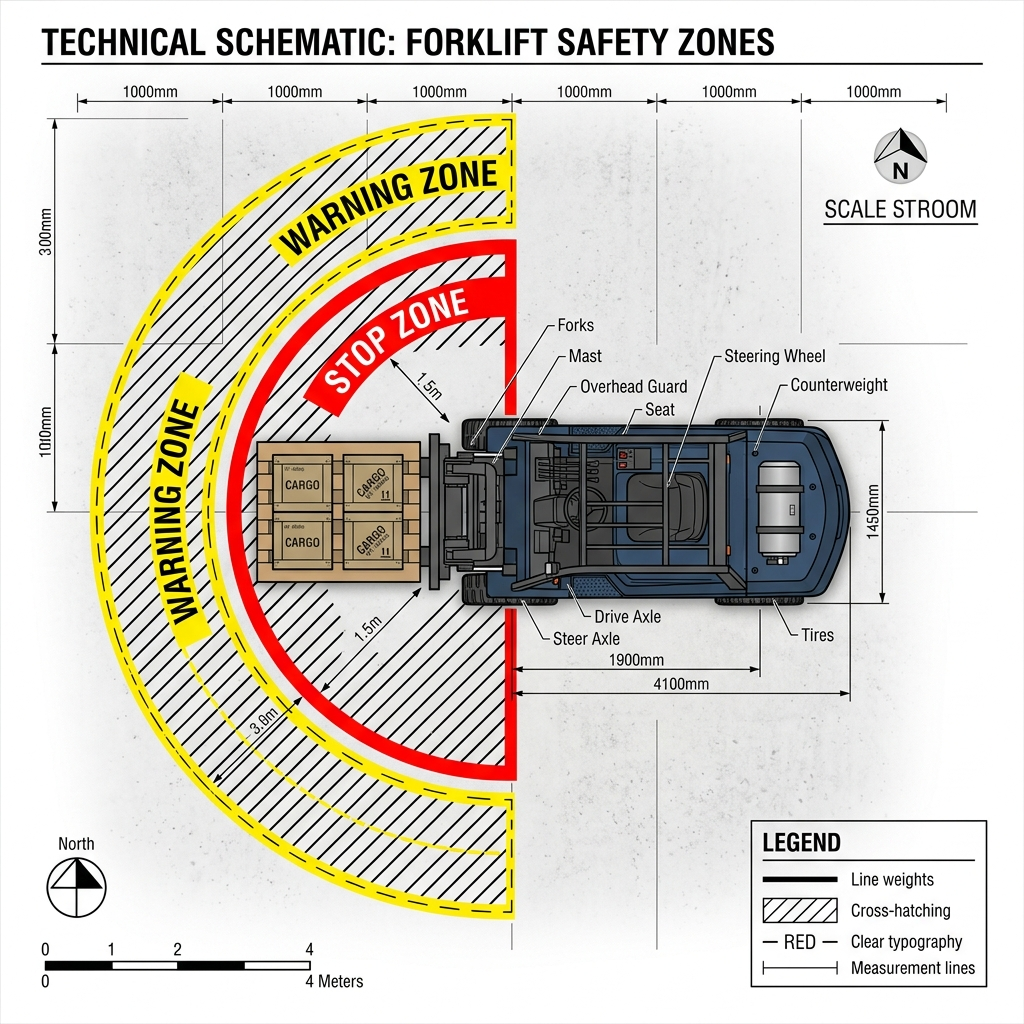
\includegraphics[width=0.6\textwidth]{slike/safety_zones.png}
\caption{Prikaz zaštitnih polja (zona upozorenja i zona zaustavljanja) oko viličara}
\label{fig:safety_zones}
\end{figure}

    \item \textbf{Taktilni branici (Bumpers):} Mehanički branici osjetljivi na pritisak koji služe kao sekundarna zaštita. Ako beskontaktni senzori ne uspiju detektirati objekt (npr. zbog zaprljanosti leća lasera), fizički pritisak na branik odmah prekida strujni krug i aktivira mehaničku kočnicu.
    \item \textbf{Vizualni i zvučni alarmi:} Vozila su opremljena zvučnim signalima, sirenama te usmjerenim plavim svjetlima (engl. \textit{Blue Spot}) koja projiciraju plavu točku na tlo nekoliko metara ispred ili iza vozila. To omogućuje pješacima u skladištu da uoče približavanje viličara iza ugla prije nego što ga fizički vide.
    \item \textbf{Tipke za hitno zaustavljanje (Emergency Stop):} Crvene gljivaste tipke montirane na lako dostupnim vanjskim mjestima šasije viličara, koje svakom radniku omogućuju trenutno mehaničko zaustavljanje stroja u slučaju opasnosti.
\end{enumerate}

\subsection{Matematički model proračuna sigurnosnih zona}
Širina i duljina sigurnosnih zona (posebno zone zaustavljanja) nisu proizvoljne, već se moraju točno izračunati za svako vozilo i radni uvjet. Formula za proračun minimalne duljine zone zaustavljanja $S$ u smjeru kretanja izražava se kao:
\begin{equation}
  S = v \cdot t_{odziv} + \frac{v^2}{2 g \mu} + d_{sig}
\end{equation}

% TODO: Dodana tablica primjera zaustavnih puteva
Tablica \ref{tab:zaustavni_put} prikazuje pojednostavljeni izračun potrebnog zaustavnog puta na temelju brzine vozila i stanja podloge (uz pretpostavku odziva sustava od $0.2$\,s).

\begin{table}[h]
\centering
\begin{tabular}{lccc}
\hline
Scenarij & v (m/s) & S (m) & Napomena \\
\hline
A & 1.0 & 1.3 & suho, $\mu=0.5$, $t_{odziv}=0.2$ s \\
B & 1.5 & 2.1 & suho, $\mu=0.5$, $t_{odziv}=0.2$ s \\
C & 2.0 & 3.5 & mokro, $\mu=0.3$, $t_{odziv}=0.2$ s \\
\hline
\end{tabular}
\caption{Primjeri zaustavnih puteva}
\label{tab:zaustavni_put}
\end{table}

Zbog toga moderni autonomni viličari integriraju sustave za dinamičku prilagodbu zona koji stalno očitavaju stanje podloge ili preventivno ograničavaju maksimalnu brzinu kretanja u zonama gdje se sumnja na lošije prianjanje kotača.
